\documentclass[a4paper,twocolumn]{article}
\usepackage[utf8]{inputenc}
\usepackage{graphicx}
\usepackage{indentfirst}
\usepackage{float}
\usepackage{fancyhdr}
\usepackage{amssymb}
\usepackage{amsmath}
\usepackage{verbatim}
\usepackage{pgfplots}
\usepackage{subcaption}
\usepackage[labelfont=bf]{caption}
\usepackage[top=2.5cm,left=1.5cm,right=1.5cm,bottom=3cm]{geometry}
\usepackage{hyperref}
\usepackage{booktabs}
\newcommand{\HRule}{\rule{\linewidth}{0.5mm}}



\begin{document}
\twocolumn[\begin{@twocolumnfalse}

\begin{center}
\large\textbf{Methods for Feature Extraction on Tiny Images for \textit{k}-Nearest Neighbors Classifiers}
\end{center}

\begin{center}
\small{Eric Miller, University of Georgia at Oxford}\\
\end{center}

\begin{center}
\small{27 June 2020}
\end{center}

\HRule \\
While low-resolution images often provide the greatest difficulty in classification problems, many cases of image recognition deal with suboptimal picture quality or size. In this paper, we explore ways in which simple models, particularly \(k\)-nearest neighbor classifiers, combined with feature extraction methods, may proficiently utilize "tiny images" in order to produce meaningful results. Certain spacial and orientation-based features prove to provide useful representations of images for classification, whereas scale invariance and keypoint recognition lose practicality at small scales. Features may also be combined in robust ways to further improve computational accuracy. \\
\HRule
\vspace{1cm}

\end{@twocolumnfalse}]

\section{Introduction}
The CIFAR-10 dataset\cite{cifar} consists of 60 thousand "tiny" images (\(32\times32\) resolution) that are separated into 10 classes of the items they represent, such as airplanes, cats, and frogs. This dataset is often used for computational image-classification problems and experiments. Baseline procedures have been performed with multiple sophisticated models, such as convolutional neural networks, but the experiments here focus on more elementary classifiers.

In addition to classification models, feature extraction algorithms---particularly for computer vision and image classificaiton---are essential in providing relevant data to simpler models. Various methods are explored in detail in order to analyze their practicality on low-resolution, "tiny" images, compared to raw-pixel value representations. Example use-cases of such low-quality image classification extends to low-cost security monitoring and satellite imaging, among a plethora of additional applications.
    
\section{Methods} 

\subsection{\textit{k}-Nearest Neighbors Model}
The central classification model was a \(k\)-nearest neighbors (\(k\)-NN) classifier. At a high level, based on a training set, additional test data can be predicted based on a table lookup, where the majority of the labels of the \(k\) closest training-set members is used for the prediction on each test-set member\cite{knn-textbook}. The freedom here lies in how "closest" is defined---both in terms of the distance metric and how the data is represented.

The \textit{k}-nearest neighbors model was implemented as a Python class, with a methods for training and testing. The \texttt{train} method simply stores the training data, while the \texttt{test} method does the brunt of the work. When the test data is loaded in, L1 distances are computed for every pair of members between the testing and training sets. The \texttt{cdist} function, which uses C-level code, from \texttt{scipy} was used in order to optimize this process.

Next, for each member of the test set, distances to training data members are sorted increasing order, and training labels are sorted accordingly. Hence, the first \textit k training labels in the sorted set can be used to vote for a label for the test data member. For simplicity and speed, \textit k may be passed into the \texttt{test} method, and distances are not recalculated or resorted if not necessary.

A separate model, which interfaced with \texttt{sklearn}'s \texttt{NearestNeighbors} module, was implemented in order to provide a baseline for runtime.

\subsection{Feature extraction}
Originally, the images were fed in as raw pixel values. However, due to the sheer size of the dataset (3072 values for each image), as well as the nature of the model, which would compare the images pixel-by-pixel and not account for invariances, feature extraction methods provided notable increases in testing accuracy. These methods transformed the image arrays into various feature arrays, upon which the model would work and calculate distances.

\subsubsection{Grayscale and Average-Value Images}
The first feature extraction method was a simple grayscale converter. As human vision has different sensitivities to different colors, those with higher sensitivity have greater weight on the grayscale image. For this purpose, the brightness value was the dot product between the RGB array (consisting of 3 floating point values between 0 and 1) and the array \texttt{[0.2989, 0.5870, 0.1140]}.

Average-value images were also created, weighing each original color equally. Both of these methods shrank the 3072-value arrays down to 1024 values. However, they were still subject to the same constraints of \textit k-NN models.

\subsubsection{Spacial Histograms}
One way to combat this issue is to create spacial histograms of pixel values. Within each specified window (e.g., the entire image, quadrants, sixteenths, etc.), and for each color (red, green, and blue), a histogram was calculated for the distribution of the color's brightness across all pixels in the window.

The variable parameters here are window size as well as bin size for the histograms. As window size and bin size increase indefinitely, the spacial histogram gets closer to the raw image, represented in a different (more verbose) format.

Theoretically, this fixes the earlier problem of using raw images (to an extent): instead of comparing raw pixels to pixels in the same locations, distributions of pixel values for each color are compared across general regions.

\subsubsection{Histogram of Oriented Gradients}
In image processing and computer vision, discrete derivatives/gradients are often used for edge detection. Large gradients indicate a strong linear shift in lighting, often indicating the presence of an edge or other feature. A Histogram of Oriented Gradients (HoG) is a common way of storing the distribution of gradient vectors throughout an image.

The first step to this is determining a grid size, which was fixed at \(8\times8\) pixel squares (forming a \(4\times4\) grid). Within each square, the gradient is calculated for each pixel. The direction derivative is defined as \[D_{\vec{u}}f(\vec{x})\lim_{h\to 0}\frac{f(\vec{x}+h\vec{u})-f(\vec{x})}{h}.\] For \(\vec{u}=\hat{\textbf \i}\), the directional derivative (also the partial derivative with respect to \(x\)) can be discretized as \((f((x,y)+(2,0))-f(x,y))/2\) with \(h=2\) (the smallest distance that avoids half-steps when centering). If we ignore the scale by half (since we care only about directions and relative magnitudes of the gradient), and shift by one, we get the partial derivative \(f_x\approx f(x+1,y)-f(x-1,y)\), which can be represented by the convolution given by kernel \([-1\;0\;1]\). Similarly, for the \(y\) partial, the kernel \([-1\;0\;1]^\top\) may be used.

These convolutions are applied across the images (with 0-padded edges to retain shape) in order to obtain \(8\times8\) matrices of the \(x\) and \(y\) gradients. These are converted to polar coordinates, producing a magnitude and direction for the gradient centered at each of the 64 pixels. Either signed gradients (between -180 and 180) or unsigned gradients (modding by 180, so opposite gradients are represented the same) may be used. This is done for each color, and, for each pixel, the polar tuple with the largest magnitude is used. A histogram is then computed for the directions throughout the square, weighted by their respective magnitudes.

Once each square in the grid is assigned a histogram, they are normalized in groups. Each adjacent \(2\times2\) block of these squares (consisting of \(16\times16\) pixels) is normalized. In a \(32\times32\) resolution image (with a \(4\times4\) grid) there are \(3\times3=9\) possible placements for the normalization block. Within each block, the four histograms are concatenated and normalized (with an L2 norm) in order to account for differences in lighting. All of the normalized histograms are hence concatenated into a single array.

\subsubsection{SIFT}
Scale-Invariant Feature Transform (SIFT) is often used for such methods of feature detection and image or sub-image classification. While the original method usually involves key-point detection through a Laplacian of Gaussian filter at multiple scales, this did not prove worthwhile for low-quality, small images with few detectable key-points.

Instead, each image was split into a \(4x4\) grid, and the center of each block was considered a key-point, and the orientation was calculated in a similar way to the original SIFT method. The same gradient method described for HoG extraction was used to provide matrices of gradient magnitudes and directions for the image. WIthin each block, the key-point direction was considered the weighted average of the directions for all gradients with magnitude at least 80\% of the maximum magnitude within the block.

Next, using OpenCV's \texttt{cv2.xfeatures2d} SIFT methods, SIFT features---the concatenation of gradient histograms within a region around each key-point, rotated against the key-point's direction---were computed. The \texttt{sklearn.cluser.KMeans} module was used on all the histograms from training data's SFIT features to form a bag of visual words model on the histograms with 500 clusters (500 different possible classifications). For each image, a 500-bin histogram was computed based on which cluster the \texttt{KMeans} model predicted for each SIFT feature.

\subsection{Concatenating Multiple Features}
Beyond individual feature extraction methods, multiple feature-extraction arrays may be concatenated in order to potentially provide the benefits of multiple methods. Firstly, the case of two feature vectors were considered. For even weighting, both feature vectors, containing all images, were L1 normalized (in order to comply mathematically with the norm metric used in the classifier), and the same norms for training data were used for the test vectors in order to provide consistency.

Next, a weight-search algorithm was used to find ideal multipliers for the two feature vectors. 5\% of both training sets were used as validation data, and the weight space was evaluated as \(\{(w_1,w_2)\mid w_1+w_2=1\}\) (all weight values are scalar multiples of this). The starting multipliers were \((.5,.5)\), and a hill climbing search, dependent on cross-validation accuracy, was implemented on \(w_2\) (\(w_1\) could be calculated accordingly). Left and right successors were considered half-way between the current value of \(w_2\) and both the lower and upper bounds, respectively. The bounds started as \([0,1]\), and any upward/downward step updated the lower/upper bound (respectively) to the previous value. A maximum of 5 steps were implemented, but the search would end early if both successor weights produced cross-validation accuracy lower than that of the current weight.

Afterwards, the two weights were scalar-multiplied in order to scale \(w_1\) to 1. The multiples were stored for later use on test-data. The first two training feature vectors were scaled by these weights, and a third feature (if applicable) could be concatenated to the end of this vector using the same method. Since \(w_1\) is always \(1\), there was no need to update the original weights of the first two features, and \(w_2\) applied to the weight of the third feature. This could be applied recursively.

\subsection{Performance Metrics}
The baseline accuracy of a random classifier over the 10 uniform classes of images is 10\%. Performance is measured in terms of top-1 accuracy for the \(k\)-NN model, only including the first-choice class prediction.

\section{Results and Analysis}

\subsection{\textit k-NN Model}
The custom \textit k-NN completed training and testing for the entire dataset in a total of 2033 seconds, compared to 1984 seconds for the \texttt{sklearn} version. As expected, both models produced the same output for various test data and values of \(k\).

%no_extract
\begin{figure}[H]
    \centering
    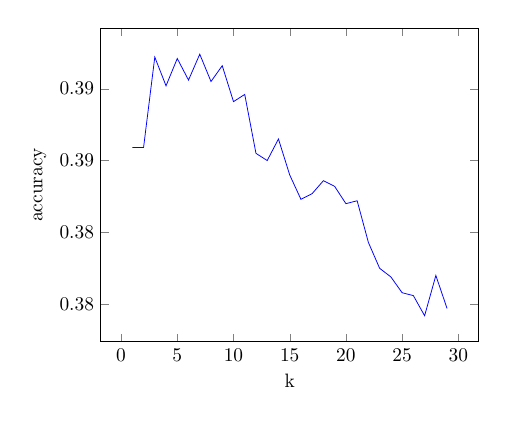
\begin{tikzpicture}[scale=.7]
        \begin{axis}[
            xlabel=k,
            ylabel=accuracy
        ]
        \addplot+[
            mark=none,
        ] plot coordinates{
            (1,0.3859)
            (2,0.3859)
            (3,0.3922)
            (4,0.3902)
            (5,0.3921)
            (6,0.3906)
            (7,0.3924)
            (8,0.3905)
            (9,0.3916)
            (10,0.3891)
            (11,0.3896)
            (12,0.3855)
            (13,0.385)
            (14,0.3865)
            (15,0.384)
            (16,0.3823)
            (17,0.3827)
            (18,0.3836)
            (19,0.3832)
            (20,0.382)
            (21,0.3822)
            (22,0.3793)
            (23,0.3775)
            (24,0.3769)
            (25,0.3758)
            (26,0.3756)
            (27,0.3742)
            (28,0.377)
            (29,0.3747)
        };
        \end{axis}
    \end{tikzpicture}
    \caption{Accuracy of \textit k-NN with raw pixel values.}
    \label{no_extract}
\end{figure}

Figure \ref{no_extract} shows that, with raw pixel values, the accuracy peaks just below 40\% with 7 nearest-neighbors, and quickly drops off above 10 nearest-neighbors. This early drop-off is likely do to the specificity of the metric, requiring similar pixels to be in the same positions, and there are rarely more than a handful of images that are truly close in value, even within the same class.

\subsection{Feature Extraction}

\subsubsection{Grayscale and Average-Value}

As Figure \ref{grayscale} shows, average-value and grayscale image reductions notably decrease classifier quality. This is a result of reduced information, as the new images contain one third of the data as the original, while still using the same fallible metric.

%grayscale
\begin{figure}[H]
    \centering
    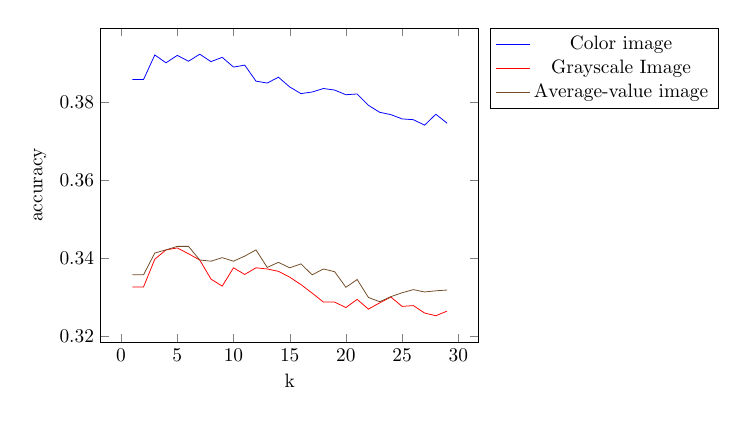
\begin{tikzpicture}[scale=.7]
        \begin{axis}[
            xlabel=k,
            ylabel=accuracy,
            legend pos=outer north east
        ]
        \addplot+[
            mark=none,
        ] plot coordinates{
            (1,0.3859)
            (2,0.3859)
            (3,0.3922)
            (4,0.3902)
            (5,0.3921)
            (6,0.3906)
            (7,0.3924)
            (8,0.3905)
            (9,0.3916)
            (10,0.3891)
            (11,0.3896)
            (12,0.3855)
            (13,0.385)
            (14,0.3865)
            (15,0.384)
            (16,0.3823)
            (17,0.3827)
            (18,0.3836)
            (19,0.3832)
            (20,0.382)
            (21,0.3822)
            (22,0.3793)
            (23,0.3775)
            (24,0.3769)
            (25,0.3758)
            (26,0.3756)
            (27,0.3742)
            (28,0.377)
            (29,0.3747)
        };
        \addlegendentry{Color image}
        \addplot+[
            mark=none,
        ] plot coordinates{
            (1,0.3327)
            (2,0.3327)
            (3,0.3398)
            (4,0.3422)
            (5,0.3427)
            (6,0.3412)
            (7,0.3396)
            (8,0.3347)
            (9,0.3329)
            (10,0.3376)
            (11,0.3359)
            (12,0.3376)
            (13,0.3373)
            (14,0.3367)
            (15,0.3352)
            (16,0.3333)
            (17,0.3311)
            (18,0.3288)
            (19,0.3288)
            (20,0.3274)
            (21,0.3295)
            (22,0.327)
            (23,0.3286)
            (24,0.3301)
            (25,0.3277)
            (26,0.3279)
            (27,0.326)
            (28,0.3253)
            (29,0.3265)
        };
        \addlegendentry{Grayscale Image}
        \addplot+[
            mark=none
        ] plot coordinates {
            (1,0.3358)
            (2,0.3358)
            (3,0.3414)
            (4,0.3422)
            (5,0.3431)
            (6,0.3431)
            (7,0.3396)
            (8,0.3393)
            (9,0.3402)
            (10,0.3393)
            (11,0.3406)
            (12,0.3422)
            (13,0.3377)
            (14,0.339)
            (15,0.3376)
            (16,0.3386)
            (17,0.3358)
            (18,0.3373)
            (19,0.3366)
            (20,0.3326)
            (21,0.3346)
            (22,0.33)
            (23,0.3289)
            (24,0.3302)
            (25,0.3312)
            (26,0.332)
            (27,0.3314)
            (28,0.3317)
            (29,0.3319)
        };
        \addlegendentry{Average-value image}
        \end{axis}
    \end{tikzpicture}
    \caption{Accuracy on color versus grayscale and average-value images.}
    \label{grayscale}
\end{figure}

\subsubsection{Spacial Histograms}

Figure \ref{hist} shows changes in accuracy resulting from increasing both window size (a) and bin size (b) for spacial histograms.

%hist
\begin{figure}[H]
    \centering
    \begin{subfigure}{0.5\textwidth}
        \centering
        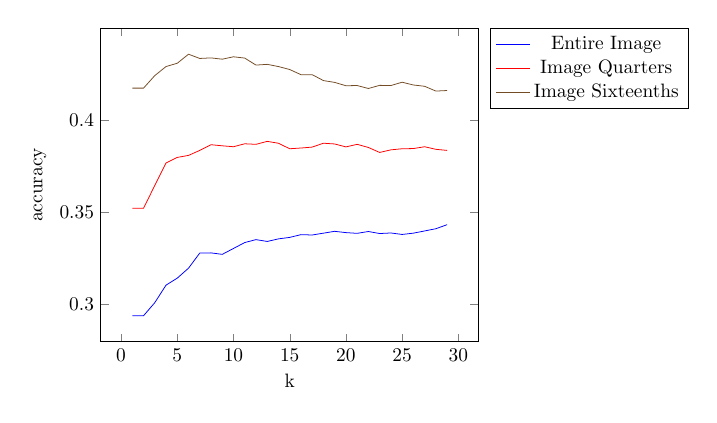
\begin{tikzpicture}[scale=.7]
            \begin{axis}[
                xlabel=k,
                ylabel=accuracy,
                legend pos=outer north east
            ]
            \addplot+[
                mark=none,
            ] plot coordinates{
                (1,0.2937)
                (2,0.2937)
                (3,0.3008)
                (4,0.3103)
                (5,0.3141)
                (6,0.3195)
                (7,0.3277)
                (8,0.3278)
                (9,0.327)
                (10,0.3302)
                (11,0.3334)
                (12,0.335)
                (13,0.334)
                (14,0.3354)
                (15,0.3362)
                (16,0.3377)
                (17,0.3375)
                (18,0.3385)
                (19,0.3395)
                (20,0.3388)
                (21,0.3384)
                (22,0.3394)
                (23,0.3383)
                (24,0.3386)
                (25,0.3378)
                (26,0.3385)
                (27,0.3397)
                (28,0.3409)
                (29,0.3431)
            };
            \addlegendentry{Entire Image};
            \addplot+[
                mark=none,
            ] plot coordinates{
                (1,0.352)
                (2,0.352)
                (3,0.3644)
                (4,0.3766)
                (5,0.3796)
                (6,0.3807)
                (7,0.3834)
                (8,0.3865)
                (9,0.3859)
                (10,0.3854)
                (11,0.387)
                (12,0.3867)
                (13,0.3883)
                (14,0.3873)
                (15,0.3843)
                (16,0.3847)
                (17,0.3852)
                (18,0.3873)
                (19,0.3869)
                (20,0.3853)
                (21,0.3867)
                (22,0.385)
                (23,0.3823)
                (24,0.3837)
                (25,0.3843)
                (26,0.3844)
                (27,0.3854)
                (28,0.384)
                (29,0.3834)
            };
            \addlegendentry{Image Quarters};
            \addplot+[
                mark=none,
            ] plot coordinates{
                (1,0.4172)
                (2,0.4172)
                (3,0.424)
                (4,0.4289)
                (5,0.4307)
                (6,0.4356)
                (7,0.4333)
                (8,0.4336)
                (9,0.4329)
                (10,0.4342)
                (11,0.4335)
                (12,0.4297)
                (13,0.4301)
                (14,0.4289)
                (15,0.4273)
                (16,0.4245)
                (17,0.4245)
                (18,0.4213)
                (19,0.4203)
                (20,0.4185)
                (21,0.4186)
                (22,0.417)
                (23,0.4187)
                (24,0.4186)
                (25,0.4204)
                (26,0.4189)
                (27,0.4182)
                (28,0.4156)
                (29,0.4159)
            };
            \addlegendentry{Image Sixteenths};
            \end{axis}
        \end{tikzpicture}
        \caption{Fixed bin size of 16, with varying window size.\\~\\~\\}
    \end{subfigure}

    \begin{subfigure}{0.5\textwidth}
        \centering
        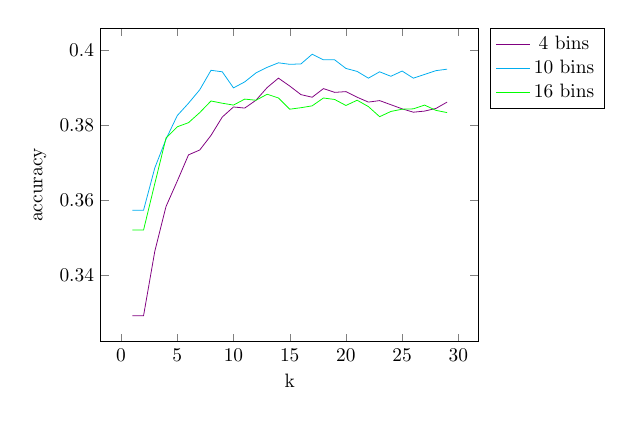
\begin{tikzpicture}[scale=.7]
            \begin{axis}[
                xlabel=k,
                ylabel=accuracy,
                legend pos=outer north east
            ]
            \addplot+[
                mark=none,
                color=violet
            ] plot coordinates{
                (1,0.3291)
                (2,0.3291)
                (3,0.3463)
                (4,0.3583)
                (5,0.3651)
                (6,0.3721)
                (7,0.3734)
                (8,0.3773)
                (9,0.3822)
                (10,0.3849)
                (11,0.3846)
                (12,0.3867)
                (13,0.3901)
                (14,0.3926)
                (15,0.3905)
                (16,0.3882)
                (17,0.3875)
                (18,0.3898)
                (19,0.3888)
                (20,0.389)
                (21,0.3875)
                (22,0.3862)
                (23,0.3866)
                (24,0.3855)
                (25,0.3844)
                (26,0.3835)
                (27,0.3838)
                (28,0.3845)
                (29,0.3862)
            };
            \addlegendentry{4 bins}
            \addplot+[
                mark=none,
                color=cyan
            ] plot coordinates{
                (1,0.3573)
                (2,0.3573)
                (3,0.3686)
                (4,0.3763)
                (5,0.3826)
                (6,0.3859)
                (7,0.3895)
                (8,0.3947)
                (9,0.3943)
                (10,0.39)
                (11,0.3916)
                (12,0.394)
                (13,0.3955)
                (14,0.3967)
                (15,0.3963)
                (16,0.3964)
                (17,0.399)
                (18,0.3975)
                (19,0.3975)
                (20,0.3952)
                (21,0.3944)
                (22,0.3926)
                (23,0.3943)
                (24,0.3931)
                (25,0.3945)
                (26,0.3926)
                (27,0.3936)
                (28,0.3946)
                (29,0.395)
            };
            \addlegendentry{10 bins}
            \addplot+[
                mark=none,
                color=green
            ] plot coordinates{
                (1,0.352)
                (2,0.352)
                (3,0.3644)
                (4,0.3766)
                (5,0.3796)
                (6,0.3807)
                (7,0.3834)
                (8,0.3865)
                (9,0.3859)
                (10,0.3854)
                (11,0.387)
                (12,0.3867)
                (13,0.3883)
                (14,0.3873)
                (15,0.3843)
                (16,0.3847)
                (17,0.3852)
                (18,0.3873)
                (19,0.3869)
                (20,0.3853)
                (21,0.3867)
                (22,0.385)
                (23,0.3823)
                (24,0.3837)
                (25,0.3843)
                (26,0.3844)
                (27,0.3854)
                (28,0.384)
                (29,0.3834)
            };
            \addlegendentry{16 bins}
            \end{axis}
        \end{tikzpicture}
        \caption{Varying bin size, with fixed window size (image quarters).}
    \end{subfigure}
    \caption{Spatial histogram feature extraction results.}
    \label{hist}
\end{figure}

When window size decreases, within the higher ranges (whole, quarters, sixteenths), classifying accuracy increases. This is likely a biproduct of there being more data, and the pixel values describing more focused regions. As expressed with raw pixel values (the extreme case), accuracy would eventually decrease with smaller window sizes, due to the fact that the windows become to focused. Hence, a medium must be found between large windows, which allow for some translation invariance, and smaller images, which provide more specific data.

Also as expected, using 10 bins performed better than using four. However, accuracy decreased when using 16 bins. This can possibly be explained by the fact that as histograms become more sparse, similar values become harder to match across images. Similar pixel values are more likely to get split into different (adjacent) bins as the bins increase, and nearest-neighbor models do not account for values being in bins close together.

Multiple instances of spacial histograms performed better than raw pixel values, and the 16-bin case with window size of image sixteenths (\(8\times8\) windows) was used for later concatenation methods.

\subsubsection{Histogram of Oriented Gradients}

The next question was whether additional features, besides simple raw pixel values or counts, could further increase the accuracy. As Figure \ref{hog} shows, using Histograms of Oriented Gradients, a more descriptive extractor in terms of \textit{k}-NN models, provided drastically stronger accuracies, barely surpassing 50\%.

%hog
\begin{figure}[H]
    \centering
    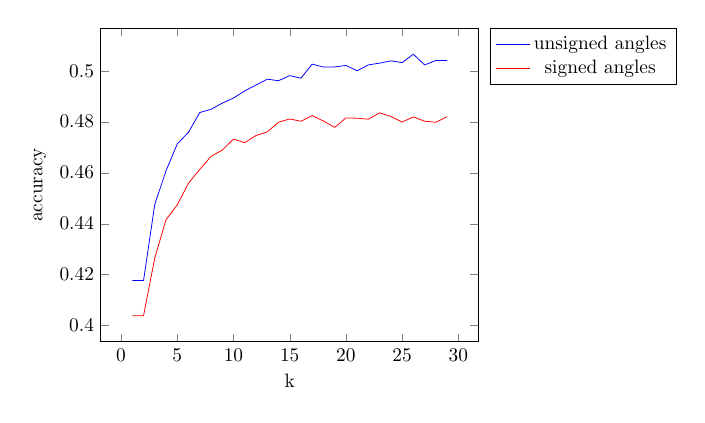
\begin{tikzpicture}[scale=.7]
        \begin{axis}[
            xlabel=k,
            ylabel=accuracy,
            legend pos=outer north east
        ]
        \addplot+[
            mark=none,
        ] plot coordinates{
            (1,0.4177)
            (2,0.4177)
            (3,0.4476)
            (4,0.4608)
            (5,0.4713)
            (6,0.4759)
            (7,0.4836)
            (8,0.4849)
            (9,0.4873)
            (10,0.4893)
            (11,0.4921)
            (12,0.4944)
            (13,0.4967)
            (14,0.4961)
            (15,0.4981)
            (16,0.4971)
            (17,0.5026)
            (18,0.5015)
            (19,0.5015)
            (20,0.5021)
            (21,0.5)
            (22,0.5023)
            (23,0.503)
            (24,0.5039)
            (25,0.5032)
            (26,0.5065)
            (27,0.5023)
            (28,0.504)
            (29,0.504)
        };
        \addlegendentry{unsigned angles}
        \addplot+[
            mark=none,
        ] plot coordinates{
            (1,0.4039)
            (2,0.4039)
            (3,0.4266)
            (4,0.4416)
            (5,0.4474)
            (6,0.4559)
            (7,0.4613)
            (8,0.4664)
            (9,0.4689)
            (10,0.4732)
            (11,0.4718)
            (12,0.4746)
            (13,0.476)
            (14,0.4798)
            (15,0.4811)
            (16,0.4802)
            (17,0.4824)
            (18,0.4803)
            (19,0.4778)
            (20,0.4815)
            (21,0.4814)
            (22,0.481)
            (23,0.4835)
            (24,0.4821)
            (25,0.4799)
            (26,0.4819)
            (27,0.4802)
            (28,0.4798)
            (29,0.482)
        };
        \addlegendentry{signed angles}
        \end{axis}
    \end{tikzpicture}
    \caption{Histogram of Oriented Gradients Extraction.}
    \label{hog}
\end{figure}

The use of unsigned angles also performed notably better than signed angles for gradients. This indicates that transitions from light to dark should not be distinguished their inverses, and that the direction of the edge itself and prominence (magnitude) of the gradient are of key importance.

\subsubsection{SIFT}

Figure \ref{sift} plots the accuracies of the SIFT extraction method.

%sift
\begin{figure}[H]
    \centering
    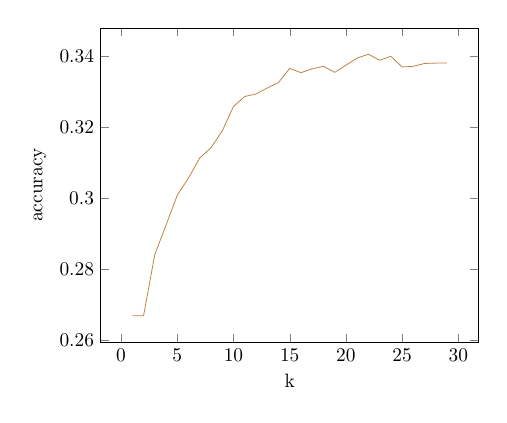
\begin{tikzpicture}[scale=.7]
        \begin{axis}[
            xlabel=k,
            ylabel=accuracy
        ]
        \addplot+[
            mark=none,
            color=brown
        ] plot coordinates{
            (1,0.2669)
            (2,0.2669)
            (3,0.2841)
            (4,0.2924)
            (5,0.3008)
            (6,0.3057)
            (7,0.3113)
            (8,0.3142)
            (9,0.3189)
            (10,0.3258)
            (11,0.3286)
            (12,0.3293)
            (13,0.331)
            (14,0.3325)
            (15,0.3365)
            (16,0.3353)
            (17,0.3364)
            (18,0.3371)
            (19,0.3354)
            (20,0.3374)
            (21,0.3394)
            (22,0.3405)
            (23,0.3388)
            (24,0.3399)
            (25,0.3369)
            (26,0.3371)
            (27,0.3379)
            (28,0.338)
            (29,0.338)
        };
        \end{axis}
    \end{tikzpicture}
    \caption{Accuracy of SIFT method.}
    \label{sift}
\end{figure}

SIFT performed notably worse than raw-pixel values. This is likely due to the fact that SIFT works best on larger resolution images, and the fact that keypoints had fixed positions on every image, but this will be explored further in the Discussion section.

\subsection{Concatenation of Multiple Features}

Figure \ref{concat_steps} shows an example of the weight decision hill-climbing search, for the concatenation of the grayscale and HoG features. With a .5:.5 (or 1:1) ratio for weights, the accuracy on a validation set was below 46\%, but increased to above 50\% and eventually surpassed pure HoG accuracy.

%concat_steps
\begin{figure}[H]
    \centering
    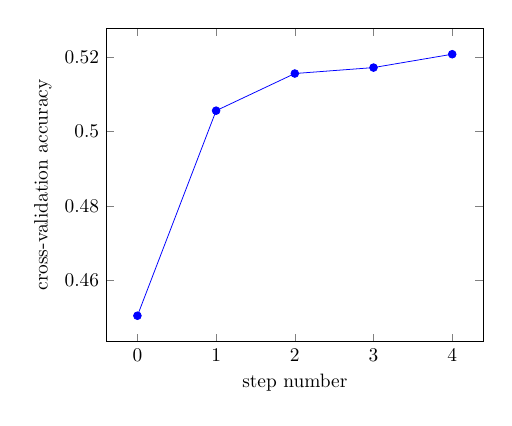
\begin{tikzpicture}[scale=.7]
        \begin{axis}[
            xlabel=step number,
            ylabel=cross-validation accuracy
        ]
        \addplot[
            color=blue,
            mark=*
        ] plot coordinates{
            (0, 0.4504)
            (1, 0.5056)
            (2, 0.5156)
            (3, 0.5172)
            (4, 0.5208)
        };
        \end{axis}
    \end{tikzpicture}
    \caption{Steps of hill climbing search for concatenation weights.}
    \label{concat_steps}
\end{figure}

In the instance that produced the above graph, the first three steps were all movements toward right-side successors (greater multiplier values for the second feature, HoG), whereas the fourth step slightly decreased the weight of the HoG feature, choosing a left successor. A fifth step was not implemented, as both the left and right successors had lower accuracies. As shown in the following graph (on the first bar), test-set accuracy was represented well by cross-validation accuracy at the final step.

%concat_bar
\begin{figure}[H]
    \centering
    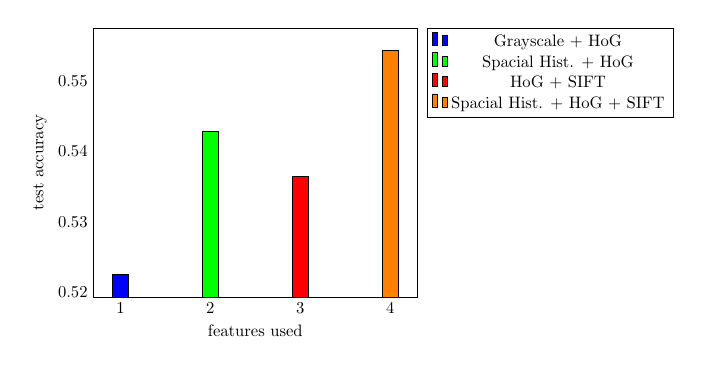
\begin{tikzpicture}[scale=.6]
        \begin{axis}[
            legend pos=outer north east,
            ylabel=test accuracy,
            xlabel=features used,
            symbolic x coords={1,,2,,3,,4},
            xtick style = {draw=none},
            ytick style = {draw=none},
            legend style={ybar legend}
        ]
        \addplot[
            ybar,
            fill=blue
        ] plot coordinates{
            (1, 0.5225)
        };
        \addlegendentry{Grayscale + HoG}
        \addplot[
            fill=green,
            ybar
        ] plot coordinates{
            (2, 0.5428)
        };
        \addlegendentry{Spacial Hist. + HoG}
        \addplot[
            fill=red,
            ybar
        ] plot coordinates{
            (3, 0.5365) %unknown
        };
        \addlegendentry{HoG + SIFT}
        \addplot[
            fill=orange,
            ybar
        ] plot coordinates{
            (4, 0.5543) %unknown
        };
        \addlegendentry{Spacial Hist. + HoG + SIFT}
        \end{axis}
    \end{tikzpicture}
    \caption{Accuracies of feature concatenation methods.}
    \label{concat_bar}
\end{figure}

Figure \ref{concat_bar} shows the accuracy of four different permutations of concatenated features (concatenated in the order shown in the legend). Note that the order of performance of concatenated features corresponds to the accuracies of the individual features used (i.e., for the first three bars, grayscale alone performed worse than SIFT, which performed worse than spacial histograms. This is reflected when concatenated with the HoG features.) Additionally, the concatenated features all performed better than the maximum of their individual parts.

%concat_table
\begin{table}[H]
    \centering
    \scalebox{0.8}{
    \begin{tabular}{llcc}
    \toprule
     & & \multicolumn{2}{c}{Multiplier} \\
     \cmidrule{3-4}
     Model & Feature & Original & Whole-Number \\ 
    \midrule
    1  & Grayscale & 1 & 3 \\
     & HoG & 9.67 & 29 \\
     \midrule
    2  & Spacial Histogram & 1 & 1 \\
     & HoG & 3 & 3 \\ 
     \midrule
    3  & HoG & 1 & 3 \\
     & SIFT & 0.33 & 1 \\ 
     \midrule
    4  & Spacial Histogram & 1 & 3 \\
     & HoG & 3 & 9 \\ 
     & SIFT & 0.33 & 1 \\ 
    \bottomrule
    \end{tabular}
    }
    \caption{Multiplier Ratios} 
    \label{concat_table}
\end{table}

Table \ref{concat_table} shows the multipliers that were calculated (and whole number ratios) for the concatenation of features, in the same order which they are shown in the histogram. Note that, for the last version, the ratio of HoG to SIFT (9:1) is different than it was in the third version (3:1). This indicates that order of the features matters when there are more than two, since if HoG and SIFT features were concatenated before the spacial histogram feature, the ratio would have been (3:1).

This is partially due to the fact that the hill-climbing algorithm went through a discretized version of the weight space, with only a limited number of possible values. However, additional possibilities are discussed in the following section.

\section{Discussion}
Compared to the baseline of 10\% accuracy from random classification, most \(k\)-NN classification methods worked relatively well. Even with raw pixel-value comparisons, which are subject to many flaws, nearly \(40\%\) accuracy was achieved. Image filters, such as grayscale and average pixel values, tended to decrease results, but also decreased memory consumption and runtime. Shifts to other image representations, such as spacial histograms, proved particularly useful in improving accuracy to above \(40\%\), and the use of more sophisticated gradient-based metrics, like Histograms of Oriented Gradients, allowed the model to surpass \(50\% accuracy\).

On the other hand, using SIFT became counterproductive, with decreased accuracy compared to raw pixel values. While runtime for \(k\)-NN training/testing decreased due to smaller input sizes (\(500\)-value arrays), the \(k-Means\) training process tremendously lengthened runtime. Without true key-point detection and scale invariance, SIFT loses its true strengths in detecting features. With such images of low resolution (i.e., \(32\times32\)), SIFT does not perform as well as other feature extractors.

In Table \ref{concat_table}, the fact that order of concatenation affects results was noted, and this was pinned on the fact that only certain discrete values in the weight set were used. Another likely possibility is that there are multiple local maxima, in which case simulated annealing could assist in providing better results, although this would take considerably more runtime.

Another likely possibility is that considering subspaces of the weight space at a time does not produce the same gradient. In the concatenation process, only two features were concatenated at a time, so even if a global maximum were found, it would only be within the plane (with all other weights fixed at zero). In the case with three features, this limits the search to a line through that point, normal to the aforementioned plane. Although this is more efficient than searching the entire weight space, for the sake of the study, it is also most likely inaccurate. Hence, a more optimal algorithm may involve gradient descent through the entire weight space, or perhaps multi-dimensional simulated annealing if time is not an issue. 

However, as noted in the previous section, this quicker method of choosing weights for concatenation nevertheless provided notable improvements in accuracy.

As well as these potential improvements on the implemented feature extractors, additional classification models, such as support-vector machines or even simple neural networks, are conjectured to provide \(60\%\) or higher accuracy without much adjustment.

\begin{thebibliography}{1}
\bibitem{cifar}
\href{https://www.cs.toronto.edu/~kriz/learning-features-2009-TR.pdf}{Learning Multiple Layers of Features from Tiny Images}, Alex Krizhevsky, 2009.
\bibitem{knn-textbook}
Peter Norvig and Stuart J. Russell. \textit{Artificial Intelligence: A Modern Approach} (3rd ed.). 738-739.
\end{thebibliography}

\end{document}